\documentclass[
	% ,draft
	,a4paper
	% ,landscape
]{article}

\usepackage{poster.preamble}
\usepackage{lipsum}
\usepackage{standalone}% \standalonefalse

% arara: pdflatex: { synctex: no }
% arara: latexmk: { clean: partial }
\begin{document}

\begin{multicols}{2}
\raggedcolumns

\begin{algorithm}[H]
	\caption{Fibonacci}
	%&../preamble

% \documentclass[varwidth=6in]{standalone}
% \usepackage{../preamble}

% arara: pdflatex: { synctex: no }
% arara: latexmk: { clean: partial }
\begin{document}
\ifstandalone
\NoCaptionOfAlgo
\begin{algorithm}[H]
\caption[Fibonacci Ricorsivo]{}
\fi

\prototype{\Int \fibonacciRic{\Int n}}{
	\eIf{\( n \leqslant 1 \)}{
		\Return \(1\)\;
	}{
		% \tcp{due chiamate ricorsive \(time \to \Omicron(2^n)\)}
		\Return \(\fibonacciRic{\(n-1\)} + \fibonacciRic{\(n-2\)}\)\;
	}
}

\ifstandalone
\end{algorithm}
\RestoreCaptionOfAlgo
\fi
\end{document}

	\documentclass[varwidth=6in]{standalone}
\usepackage{../_preamble}

% arara: pdflatex: { synctex: no }
% arara: latexmk: { clean: partial }
\begin{document}
\ifstandalone
\NoCaptionOfAlgo
\begin{algorithm}[H]
\caption[Fibonacci iterativo]{}
\fi

\prototype{\Int \fibonacciIter{\Int \(n\)}}{

	\BlankLine
	\(DP\) \Assign \new \Array{\Int}{0}{n}\;
	\ArrayCall{DP}{0} \Assign \ArrayCall{DP}{1} \Assign 1\;

	\BlankLine
	\From{\(i \Assign 2\) \DownTo \(n\)}{
		\ArrayCall{DP}{i} \Assign \(\ArrayCall{DP}{i-1} + \ArrayCall{DP}{i-2}\)\;
	}

	\BlankLine
	\Return \ArrayCall{DP}{n}\;
}

\ifstandalone
\end{algorithm}
\RestoreCaptionOfAlgo
\fi
\end{document}

	%&../preamble

% arara: pdflatex: { synctex: no }
% arara: latexmk: { clean: partial }
\ifstandalone
\begin{document}
\begin{algorithm}[H]
\fi

\prototype{\Int \fibonacci{\Int n}}{
	\Int \(DP_0 \Assign 1\)\;
	\Int \(DP_1 \Assign 1\)\;
	\Int \(DP_2 \Assign 1\)\;

	\BlankLine
	\From{\(i \Assign 2\) \DownTo \(n\)}{
		\(DP_0 \Assign DP_1\)\;
		\(DP_1 \Assign DP_2\)\;
		\(DP_2 \Assign DP_0 + DP_1\)\;
	}

	\Return \(DP_2\)\;
}

\ifstandalone
\end{algorithm}
\end{document}
\fi

\end{algorithm}

\paragraph{Fibonacci}
Lorem ipsum dolor sit amet, consectetur adipisicing elit, sed do eiusmod tempor incididunt ut labore et dolore magna aliqua. Ut enim ad minim veniam, quis nostrud exercitation ullamco laboris nisi ut aliquip ex ea commodo consequat. Duis aute irure dolor in reprehenderit in voluptate velit esse cillum dolore eu fugiat nulla pariatur. Excepteur sint occaecat cupidatat non proident, sunt in culpa qui officia deserunt mollit anim id est laborum.
lorem

\begin{algorithm}[H]
	\caption{Codice di Huffman}
	\documentclass[varwidth=6in]{standalone}
\usepackage{../_preamble}

% arara: pdflatex: { synctex: no }
% arara: latexmk: { clean: partial }
\begin{document}
\ifstandalone
\NoCaptionOfAlgo
\begin{algorithm}[H]
\caption[Algoritmo di Huffman]{}
\fi

\prototype{\Tree \huffman{\Array{\Int} \(c\), \Array{\Int} \(f\), \Int \(n\)}}{
	\tcp{\Array{c}{1}{n}: caratteri dell'alfabeto}
	\tcp{\(f[1 \dots n]\): frequenze dei caratteri}
	\tcp{\(n\): dimensione dell'alfabeto}

	\BlankLine
	\Heap \(Q\) \Assign \minHeapConstructor\;

	\BlankLine
	\From(\Comment*[h]{}{\(\Omicron(n)\)}){\(i \Assign 1\) \DownTo \(n\)}{
		\(Q\).\heapInsert{\(f[i]\), \treeConstructor{\(f[i]\), \(c[i]\)}} \Comment*[h]{}{\(\Omicron(\log n)\)}
	}

	\BlankLine
	\From(\Comment*[h]{\(n\): radice}{\(\Omicron(n)\)}){\(i \Assign 1\) \DownTo \(n-1\)}{
		\BlankLine
		\tcp{estraggo i 2 caratteri meno frequenti}
		\(z_1\) \Assign \(Q\).\heapDeleteMin\;
		\(z_2\) \Assign \(Q\).\heapDeleteMin\;

		\BlankLine
		\tcp{Creo un nuovo nodo}
		\(z \Assign \treeConstructor(z_1.f + z_2.f, \Nil)\)\;
		\(z.\varLeft \Assign z_1\)\;
		\(z.\varRight \Assign z_2\)\;

		\BlankLine
		\tcp{Lo inserisco nella coda}
		% \marginnote{\color{blue} \(\Omicron(\log n)\)}
		\(Q\).\heapInsert{z.f, z}\;
	}

	\Return \(Q\).\heapDeleteMin\;
}

\ifstandalone
\end{algorithm}
\RestoreCaptionOfAlgo
\fi
\end{document}

\end{algorithm}

\paragraph{Codice di Huffman}
\lipsum[1-4]

\begin{algorithm}[H]
	\caption{Resto}
	\documentclass[varwidth=6in]{standalone}
\usepackage{../_preamble}

% arara: pdflatex: { synctex: no }
% arara: latexmk: { clean: partial }
\begin{document}
\ifstandalone
\NoCaptionOfAlgo
\begin{algorithm}[H]
\caption[Approccio programmazione dinamica al problema del resto]{}
\fi

\prototype{\restoDP{\Array{\Int} t, \Int n, \Int R}}{
	\tcp{\(t\): tagli disponibili,\(n\): numero di monete, \(R\) il resto da dare}

	\BlankLine
	\(DP\) \Assign \new \Array{\Int}{0}{R}\;
	\(S\) \Assign \new \Array{\Int}{0}{R}\;
	\(\ArrayCall{DP}{0} \Assign 0\) \Comment*[h]{caso base}\;

	\BlankLine
	\tcp{Riempire la tabella \(DP\)}
	\From{\(i \Assign 1\) \DownTo \(R\)} {
		\(DP[i] \Assign +\infty\)\;

		\BlankLine
		\BlankLine
		\From(\Comment*[h]{Riempio la tabella}){\(j \Assign 1\) \DownTo \(n\)} {
			\If{\(i > t[j]\) \And \(DP[i-t[j]] + 1 < DP[i]\)}{
				\tcp{aggiorno il valore}

				\BlankLine
				\(DP[i] \Assign DP[i - t[j]] + 1\) \Comment*[h]{registro il valore}\;
				\(S[i] \Assign j\) \Comment*[h]{la moneta da utilizzare per risolvere il problema quando il taglio è \(i\)}\;
			}
		}
	}

	\BlankLine
	\While(\Comment*[h]{ho resto da dare}){\(R > 0\)}{
		\Print \(t[S[R]]\) \Comment*[h]{stampo la moneta}\;
		\(R \Assign R - t[S[R]]\) \Comment*[h]{decremento il resto}\;
	}
}

\ifstandalone
\end{algorithm}
\RestoreCaptionOfAlgo
\fi
\end{document}

	%&../preamble

% \documentclass[varwidth=6in]{standalone}
% \usepackage{../preamble}

% arara: pdflatex: { synctex: no }
% arara: latexmk: { clean: partial }
\ifstandalone
\begin{document}
\NoCaptionOfAlgo
\begin{algorithm}[H]
\caption[Approccio ingordo al problema del resto]{}
\fi

\prototype{\restoGreedy{\Array{\Int} \(t\), \Int \(n\), \Int \(R\), \Array{\Int} \(x\)}}{

	\{ Ordina le monete in modo \emph{decrescente} \}\;
	\tcp{\(\Omicron(n)\) se già ordinato, \(\Omicron(n \log n)\) altrimenti}

	\BlankLine
	\From(\Comment*[h]{\(\Omicron(n)\)}){\(i \Assign 1\) \DownTo \(n\)} {

		\BlankLine
		\tcp{il numero di monete di taglio massimo}
		\(x[i] \Assign \left\lfloor \dfrac{R}{t[i]} \right\rfloor\)\;

		\BlankLine
		\tcp{calcolo il resto rimanente}
		\(R \Assign R - x[i] \cdot t[i]\)\;
	}

	\Return \(R\)
}

\ifstandalone
\end{algorithm}
\RestoreCaptionOfAlgo
\end{document}
\fi

divido il resto per il taglio della moneta più grande trovando il numero di monete massimo di quel taglio, dopodiché
tolgo il valore della somma quelle monete dal resto.

\end{algorithm}

\paragraph{Problema del resto}
Lorem ipsum dolor sit amet, consectetur adipisicing elit, sed do eiusmod tempor incididunt ut labore et dolore magna aliqua. Ut enim ad minim veniam, quis nostrud exercitation ullamco laboris nisi ut aliquip ex ea commodo consequat. Duis aute irure dolor in reprehenderit in voluptate velit esse cillum dolore eu fugiat nulla pariatur. Excepteur sint occaecat cupidatat non proident, sunt in culpa qui officia deserunt mollit anim id est laborum.

\begin{algorithm}[H]
	\caption{Zaino}
	% %&../preamble

% arara: pdflatex: { synctex: no }
% arara: latexmk: { clean: partial }
\begin{document}
\ifstandalone
\begin{algorithm}[H]
\fi

% TODO
\prototype{\Int \knapsack{\Array{\Int} \(w\), \Array{\Int} \(p\), \Int \(n\), \Int \(C\)}}{

    \BlankLine
    \tcp{comment}
    \(DP \Assign \new \Array{\Int}[0\dots n][0\dots C]\)\;

    \BlankLine
    \tcp{comment}
    ...
}

\ifstandalone
\end{algorithm}
\fi
\end{document}

	%&../preamble

% \documentclass[varwidth=6in]{standalone}
% \usepackage{../preamble}

% arara: pdflatex: { synctex: no }
% arara: latexmk: { clean: partial }
\begin{document}
\ifstandalone
\NoCaptionOfAlgo
\begin{algorithm}[H]
\caption[Zaino greedy]{}
\fi

\prototype{\zaino{\Array{\Real} \(p\), \Array{\Real} \(v\), \Real \(C\), \Int \(n\), \Array{\Real} \(x\)}}{

	\BlankLine
	\{ ordina \(p\) e \(v\) in modo che \(\frac{p[1]}{w[1]} \geqslant \frac{p[2]}{w[2]} \geqslant \cdots \geqslant \frac{p[n]}{w[n]}\)\}\;

	\BlankLine
	\tcp{\(\Omicron(n)\) se già ordinato, \(\Omicron(n \log n)\) altrimenti}

	\BlankLine
	\BlankLine
	\From{\(i \Assign 1\) \DownTo \(n\)}{
		\(x[i] \Assign \MathMin\left( \dfrac{C}{w[i]}, 1 \right)\) \Comment*[h]{ne prendo solo una frazione?}\;

		\BlankLine
		\(C \Assign C - x[i] \cdot w[i]\) \Comment*[h]{aggiorno la capacità residua}\;
	}
}

\ifstandalone
\end{algorithm}
\RestoreCaptionOfAlgo
\fi
\end{document}

\end{algorithm}

\paragraph{Problema dello zaino}
Lorem ipsum dolor sit amet, consectetur adipisicing elit, sed do eiusmod tempor incididunt ut labore et dolore magna aliqua. Ut enim ad minim veniam, quis nostrud exercitation ullamco laboris nisi ut aliquip ex ea commodo consequat. Duis aute irure dolor in reprehenderit in voluptate velit esse cillum dolore eu fugiat nulla pariatur. Excepteur sint occaecat cupidatat non proident, sunt in culpa qui officia deserunt mollit anim id est laborum.

\begin{algorithm}[H]
	\caption{Parentesizzazione}
	%&../preamble

% \documentclass[varwidth=6in]{standalone}
% \usepackage{../preamble}

% arara: pdflatex: { synctex: no }
% arara: latexmk: { clean: partial }
\ifstandalone
\begin{document}
\NoCaptionOfAlgo
\begin{algorithm}[H]
\caption[Parentesizzazione ricorsiva]{}
\fi

\prototype{\Int \recPar{\Array{\Int} c, \Int i, \Int j}}{

	\BlankLine
	\eIf(\tcp*[h]{se gli indici corrispondono}){i \Assign j}{
		\Return 0 \tcp*[h]{non devo fare operazioni}
	}{
		\(min \Assign +\infty\)\;

		\tcp{Tutta la logica dell'algoritmo}
		\From{\Int \(k \Assign i\) \DownTo \(j - 1\)}{
			\Int \(q\) \Assign \(\recPar{c, i, k} + \recPar{\(c\), \(k + 1\), \(j\)} + \Array{c}{i - 1} \cdot \Array{c}{k} \cdot \Array{c}{j}\)\;

			\BlankLine
			\If(\tcp*[h]{se \(q\) è più piccolo del minimo}){\( q < min \)}{
				\(min \Assign q\) \tcp*[h]{aggiorniamo il minimo}
			}
		}
	}
	\Return \(min\)\;
}

\ifstandalone
\end{algorithm}
\RestoreCaptionOfAlgo
\end{document}
\fi

	%&../preamble

% arara: pdflatex: { synctex: no }
% arara: latexmk: { clean: partial }
\ifstandalone
\begin{document}
\begin{algorithm}[H]
\fi

\prototype{\Matrix{\Int} \multiplyFunction{\Matrix{\Int} A, \Matrix{\Int} S, \Int i, \Int j}}{

	\BlankLine
	\eIf{\( i \Equal j \)}
	{ \Return \Array{A}{i}\; }
	{
		\BlankLine
		\Matrix{\Int} \(X\) = \multiplyFunction{\( last[][], i, last[i][j] \)}\;

		\Matrix{\Int} \(Y\) = \multiplyFunction{\( last[][], last[i][j] + 1, j \)}\;

		\BlankLine
		\Return \multiplyMatrices{X,Y}
	}
}

\ifstandalone
\end{algorithm}
\end{document}
\fi

\end{algorithm}
\paragraph{Moltiplicazione fra matrici}
Lorem ipsum dolor sit amet, consectetur adipisicing elit, sed do eiusmod tempor incididunt ut labore et dolore magna aliqua. Ut enim ad minim veniam, quis nostrud exercitation ullamco laboris nisi ut aliquip ex ea commodo consequat. Duis aute irure dolor in reprehenderit in voluptate velit esse cillum dolore eu fugiat nulla pariatur. Excepteur sint occaecat cupidatat non proident, sunt in culpa qui officia deserunt mollit anim id est laborum.

\end{multicols}

\newpage
\begin{multicols}{2}

% \begin{algorithm}[H]
% \caption{}
% \input{stringmatching}
% \end{algorithm}

\begin{algorithm}[H]
	\caption{Insieme disgiunto di intervalli pesati}
	%&../preamble

% \documentclass[varwidth=6in]{standalone}
% \usepackage{../preamble}

% arara: pdflatex: { synctex: no }
% arara: latexmk: { clean: partial }
\begin{document}
\ifstandalone
\NoCaptionOfAlgo
\begin{algorithm}[H]
\caption[Insieme indipendente di intervalli disgiunti]{}
\fi

\prototype{\Set \maxInterval{\Int a, \Int b, \Int w, \Int n}}{

	\{ ordina gli intervalli per estremi di fine crescenti \}\;

	\BlankLine
	\Matrix{\Int} \(pred\) \Assign \computePredecessor{a, b, n}\;
	\Matrix{\Int} \(DP\) \Assign \new \Array{\Int}{0}{n}\;

	\BlankLine
	\tcp{riempio la tabella}
	\(\ArrayCall{DP}{0} \Assign 0\)\;
	\From{\(i \Assign 1\) \DownTo \(n\)}{
		\ArrayCall{DP}{i} \Assign \MathMax{\(\ArrayCall{DP}{i-1}\), \(w[i] + \ArrayCall{DP}{pred[i]}\)}\;
	}

	\tcp{costruisco l'insieme dei predecessori}
	\(i \Assign n\)\;
	\Set \(S \Assign \setConstructor\)\;

	\BlankLine
	\While(\Comment*[h]{fintanto che ci sono intervalli disponibili}){\( i > 0 \)}{

		\BlankLine
		\eIf(\Comment*[h]{commento}){\(\ArrayCall{DP}{i-1} > \weight{i} + \ArrayCall{DP}{\ArrayCall{pred}{i}}\)}{
			\(\Decrement{i}\) \Comment*[h]{non considerarlo}\;
		}{
			\(S.\setInsert(i)\) \Comment*[h]{inseriscilo nell'insieme}\;
			\(i \Assign\ArrayCall{pred}{i}\) \Comment*[h]{scorri gli interalli}\;
		}
	}
	\Return \(S\) \Comment*[h]{ritorna l'insieme di intervalli ordinati}\;
}

\ifstandalone
\end{algorithm}
\RestoreCaptionOfAlgo
\fi
\end{document}

	%&../preamble

% \documentclass[varwidth=6in]{standalone}
% \usepackage{../preamble}

% arara: pdflatex: { synctex: no }
% arara: latexmk: { clean: partial }
\ifstandalone
\begin{document}
\NoCaptionOfAlgo
\begin{algorithm}[H]
\caption[Computazione dei predecessori i predecessori]{}
\fi

\tcp{Pre-computa i predecessori}
\prototype{\Array{\Int} \computePredecessor{\Array{\Int} a, \Array{\Int} a, \Int n}}{

	\BlankLine
	\Matrix{\Int} \(pred\) \(\Assign\) \new \Array{\Int}{0}{n}\;
	\(\ArrayCall{pred}{0} \Assign 0\)\;

	\BlankLine
	\From{\(i \Assign 1\) \DownTo \(n\)}{
		\(j \Assign i-1\)\;

		\BlankLine
		\While{\(j > 0\) \And \(b[j] > a[i]\)}{
			\(j \Assign j - 1\)\;
		}
		\(\ArrayCall{pred}{i} \Assign j\)\;
	}

	\BlankLine
	\Return \(pred\)\;
}

\ifstandalone
\end{algorithm}
\RestoreCaptionOfAlgo
\end{document}
\fi

	%&../preamble

% \documentclass[varwidth=6in]{standalone}
% \usepackage{../preamble}

% arara: pdflatex: { synctex: no }
% arara: latexmk: { clean: partial }
\begin{document}
\ifstandalone
\NoCaptionOfAlgo
\begin{algorithm}[H]
\caption[Insieme indipendente di intervalli disgiunti]{}
\fi

\prototype{\Set \independentSet{\Array{\Int} \(a\), \Array{\Int} \(b\)}}{

	\BlankLine
	\{ ordina \(a\) e \(b\) in modo che \(b[1] \leqslant b[2] \leqslant \cdots \le b[n]\) \}\;
	\tcp{\(\Omicron(n)\) se già ordinati, \(\Omicron(n \log n)\) altrimenti}

	\BlankLine
	\Set \(S \Assign \setConstructor\)\;
	\(S\).\setInsert(1) \Comment*[h]{inserisco il primo intervallo}\;
	\Int \Last \(\Assign 1\) \Comment*[h]{ultimo intervallo inserito}\;

	\BlankLine
	\From{\(i \Assign 2\) \DownTo \(n\)}{
		\If{\(a[i] \geqslant b[\Last]\)}{
			\tcp{gli intervalli sono indipendenti}

			\BlankLine
			\(S\).\setInsert(i) \Comment*[h]{lo inserisco}\;
			\(\Last \Assign i\) \Comment*[h]{lo rendo l'ultimo inserito}\;
		}
	}

	\Return \(S\)\;
}

\ifstandalone
\end{algorithm}
\RestoreCaptionOfAlgo
\fi
\end{document}

\end{algorithm}

\begin{figure}[H]
	\centering
	\documentclass[multi=page, tikz, border=2mm]{standalone}
\usepackage{../tikz-preamble}

% arara: pdflatex: { draft: yes }
% arara: pdflatex: { synctex: no }
% arara: latexmk:  { clean: partial }
\begin{document}

\begin{page}
	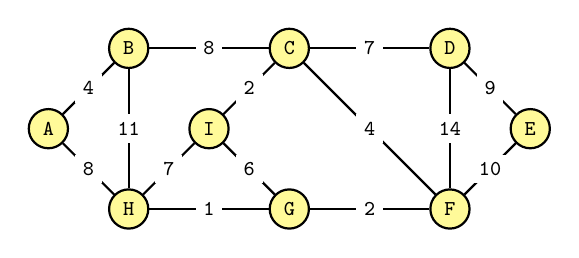
\begin{tikzpicture}[
		scale=0.85,
		transform shape,
		thick,
		font=\ttfamily\bfseries\small
	]
	\tikzset{
		mynode/.style = {circle, draw=black, align=center,fill=yellow!40},
		myedge/.style = {midway, fill=white},
		edgen/.style = {-},
		edger/.style = {-, ultra thick, red},
	}
	\node[mynode] at (0.0,1.2) (a) {A};
	\node[mynode] at (1.2,2.4) (b) {B};
	\node[mynode] at (6.0,2.4) (d) {D};
	\node[mynode] at (3.6,2.4) (c) {C};
	\node[mynode] at (1.2,0.0) (h) {H};
	\node[mynode] at (3.6,0.0) (g) {G};
	\node[mynode] at (6.0,0.0) (f) {F};
	\node[mynode] at (2.4,1.2) (i) {I};
	\node[mynode] at (7.2,1.2) (e) {E};
	%
	\draw[edgen] (a) edge node[myedge] {4} (b);
	\draw[edgen] (b) edge node[myedge] {8} (c);
	\draw[edgen] (c) edge node[myedge] {7} (d);
	\draw[edgen] (d) edge node[myedge] {9} (e);
	%
	\draw[edgen] (a) edge node[myedge] {8} (h);
	\draw[edgen] (h) edge node[myedge] {1} (g);
	\draw[edgen] (g) edge node[myedge] {2} (f);
	\draw[edgen] (f) edge node[myedge] {10} (e);
	%
	\draw[edgen] (h) edge node[myedge] {7} (i);
	\draw[edgen] (i) edge node[myedge] {6} (g);
	\draw[edgen] (i) edge node[myedge] {2} (c);
	%
	\draw[edgen] (b) edge node[myedge] {11} (h);
	\draw[edgen] (d) edge node[myedge] {14} (f);
	\draw[edgen] (c) edge node[myedge] {4} (f);
	\end{tikzpicture}
\end{page}

\begin{page}
    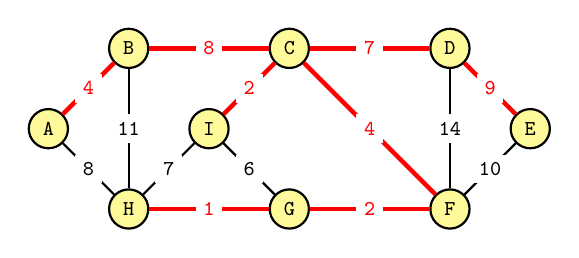
\begin{tikzpicture}[
        scale=0.85,
        transform shape,
        thick,
        font=\ttfamily\bfseries\small
    ]
    \tikzset{
        mynode/.style = {circle, draw=black, align=center,fill=yellow!40},
        myedge/.style = {midway, fill=white},
        edgen/.style = {-},
        edger/.style = {-, ultra thick, red},
    }
    \node[mynode] at (0.0,1.2) (a) {A};
    \node[mynode] at (1.2,2.4) (b) {B};
    \node[mynode] at (6.0,2.4) (d) {D};
    \node[mynode] at (3.6,2.4) (c) {C};
    \node[mynode] at (1.2,0.0) (h) {H};
    \node[mynode] at (3.6,0.0) (g) {G};
    \node[mynode] at (6.0,0.0) (f) {F};
    \node[mynode] at (2.4,1.2) (i) {I};
    \node[mynode] at (7.2,1.2) (e) {E};
    %
    \draw[edger] (a) edge node[myedge] {4} (b);
    \draw[edger] (b) edge node[myedge] {8} (c);
    \draw[edger] (c) edge node[myedge] {7} (d);
    \draw[edger] (d) edge node[myedge] {9} (e);
    %
    \draw[edgen] (a) edge node[myedge] {8} (h);
    \draw[edger] (h) edge node[myedge] {1} (g);
    \draw[edger] (g) edge node[myedge] {2} (f);
    \draw[edgen] (f) edge node[myedge] {10} (e);
    %
    \draw[edgen] (h) edge node[myedge] {7} (i);
    \draw[edgen] (i) edge node[myedge] {6} (g);
    \draw[edger] (i) edge node[myedge] {2} (c);
    %
    \draw[edgen] (b) edge node[myedge] {11} (h);
    \draw[edgen] (d) edge node[myedge] {14} (f);
    \draw[edger] (c) edge node[myedge] {4} (f);
    \end{tikzpicture}
\end{page}

\begin{page}
    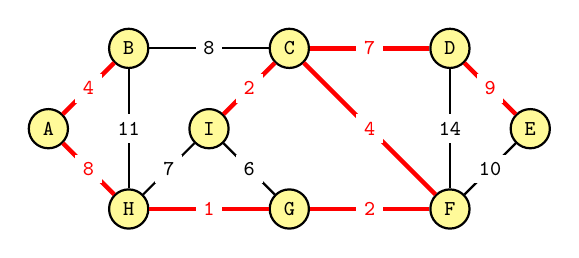
\begin{tikzpicture}[
        scale=0.85,
        transform shape,
        thick,
        font=\ttfamily\bfseries\small
    ]
    \tikzset{
        mynode/.style = {circle, draw=black, align=center,fill=yellow!40},
        myedge/.style = {midway, fill=white},
        edgen/.style = {-},
        edger/.style = {-, ultra thick, red},
    }
    \node[mynode] at (0.0,1.2) (a) {A};
    \node[mynode] at (1.2,2.4) (b) {B};
    \node[mynode] at (6.0,2.4) (d) {D};
    \node[mynode] at (3.6,2.4) (c) {C};
    \node[mynode] at (1.2,0.0) (h) {H};
    \node[mynode] at (3.6,0.0) (g) {G};
    \node[mynode] at (6.0,0.0) (f) {F};
    \node[mynode] at (2.4,1.2) (i) {I};
    \node[mynode] at (7.2,1.2) (e) {E};
    %
    \draw[edger] (a) edge node[myedge] {4} (b);
    \draw[edgen] (b) edge node[myedge] {8} (c);
    \draw[edger] (c) edge node[myedge] {7} (d);
    \draw[edger] (d) edge node[myedge] {9} (e);
    %
    \draw[edger] (a) edge node[myedge] {8} (h);
    \draw[edger] (h) edge node[myedge] {1} (g);
    \draw[edger] (g) edge node[myedge] {2} (f);
    \draw[edgen] (f) edge node[myedge] {10} (e);
    %
    \draw[edgen] (h) edge node[myedge] {7} (i);
    \draw[edgen] (i) edge node[myedge] {6} (g);
    \draw[edger] (i) edge node[myedge] {2} (c);
    %
    \draw[edgen] (b) edge node[myedge] {11} (h);
    \draw[edgen] (d) edge node[myedge] {14} (f);
    \draw[edger] (c) edge node[myedge] {4} (f);
    \end{tikzpicture}
\end{page}

\begin{page}
    \begin{tikzpicture}[
        scale=0.9,
        transform shape,
        thick,
        font=\ttfamily\bfseries\small
    ]
    \tikzset{
        mynodea/.style = {circle, draw=black, align=center,fill=yellow!40},
        mynodeb/.style = {circle, draw=black, align=center,fill=blue!40},
        myedge/.style = {midway, fill=white},
        edgen/.style = {-},
        edger/.style = {-, ultra thick, red},
        edgeb/.style = {-, ultra thick, blue},
    }
        \node[mynodeb] at (0.0,1.2) (a) {A};
        \node[mynodeb] at (1.2,2.4) (b) {B};
        \node[mynodeb] at (6.0,2.4) (d) {D};
        \node[mynodea] at (3.6,2.4) (c) {C};
        \node[mynodea] at (1.2,0.0) (h) {H};
        \node[mynodea] at (3.6,0.0) (g) {G};
        \node[mynodea] at (6.0,0.0) (f) {F};
        \node[mynodea] at (2.4,1.2) (i) {I};
        \node[mynodeb] at (7.2,1.2) (e) {E};
        %
        \draw[edger] (a) edge node[myedge] {4} (b);
        \draw[edgen] (b) edge node[myedge] {8} (c);
        \draw[edgeb] (c) edge node[myedge] {7} (d);
        \draw[edgen] (d) edge node[myedge] {9} (e);
        %
        \draw[edgen] (a) edge node[below] {8} (h);
        \draw[edger] (h) edge node[myedge] {1} (g);
        \draw[edger] (g) edge node[myedge] {2} (f);
        \draw[edgen] (f) edge node[below] {10} (e);
        %
        \draw[edgen] (h) edge node[myedge] {7} (i);
        \draw[edgen] (i) edge node[myedge] {6} (g);
        \draw[edger] (i) edge node[myedge] {2} (c);
        %
        \draw[edgen] (b) edge node[myedge] {11} (h);
        \draw[edgen] (d) edge node[myedge] {14} (f);
        \draw[edger] (c) edge node[myedge] {4} (f);

        % TAGLIO
        \path[draw, dashed] (0.2,0) .. controls (2.4,4.2) and (4.8,4.2) .. (7.0,0);

        % LEGENDA
        \node[ellipse, draw=black, align=center, fill=yellow!40, minimum width=1.5cm, anchor=west] at (8,3.0) (e) {S};
        \node[ellipse, draw=black, align=center, fill=blue!40, minimum width=1.5cm, anchor=west] at (8,2.0) (e) {V-S};
        \node[font=\sffamily, anchor=west, align=left] at (10.0,2.5) {Taglio};
        \node[font=\sffamily, anchor=west, align=left] at (10.0,1.0) {Insieme $A$};
        \node[font=\sffamily, anchor=west, align=left] at (10.0,0.0) {Arco leggero};
        \draw[ultra thick, black, dashed] (8.00,2.5) -- (9.5,2.5);
        \draw[ultra thick, red] (8.00,1.0) -- (9.5,1.0);
        \draw[ultra thick, blue] (8.00,0.0) -- (9.5,0.0);
    \end{tikzpicture}
\end{page}

\begin{page}
	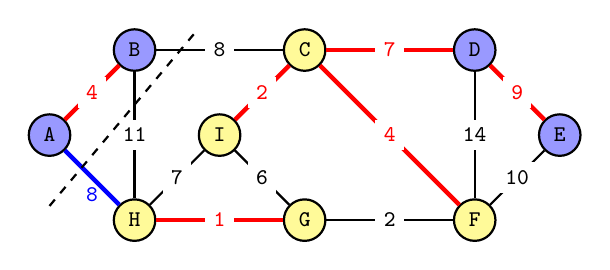
\begin{tikzpicture}[
		scale=0.9,
		transform shape,
		thick,
		font=\ttfamily\bfseries\small
	]
	\tikzset{
		mynodea/.style = {circle, draw=black, align=center,fill=yellow!40},
		mynodeb/.style = {circle, draw=black, align=center,fill=blue!40},
		myedge/.style = {midway, fill=white},
		edgen/.style = {-},
		edger/.style = {-, ultra thick, red},
		edgeb/.style = {-, ultra thick, blue},
	}
		\node[mynodeb] at (0.0,1.2) (a) {A};
		\node[mynodeb] at (1.2,2.4) (b) {B};
		\node[mynodeb] at (6.0,2.4) (d) {D};
		\node[mynodea] at (3.6,2.4) (c) {C};
		\node[mynodea] at (1.2,0.0) (h) {H};
		\node[mynodea] at (3.6,0.0) (g) {G};
		\node[mynodea] at (6.0,0.0) (f) {F};
		\node[mynodea] at (2.4,1.2) (i) {I};
		\node[mynodeb] at (7.2,1.2) (e) {E};
		%
		\draw[edger] (a) edge node[myedge] {4} (b);
		\draw[edgen] (b) edge node[myedge] {8} (c);
		\draw[edger] (c) edge node[myedge] {7} (d);
		\draw[edger] (d) edge node[myedge] {9} (e);
		%
		\draw[edgeb] (a) edge node[below] {8} (h);
		\draw[edger] (h) edge node[myedge] {1} (g);
		\draw[edgen] (g) edge node[myedge] {2} (f);
		\draw[edgen] (f) edge node[myedge] {10} (e);
		%
		\draw[edgen] (h) edge node[myedge] {7} (i);
		\draw[edgen] (i) edge node[myedge] {6} (g);
		\draw[edger] (i) edge node[myedge] {2} (c);
		%
		\draw[edgen] (b) edge node[myedge] {11} (h);
		\draw[edgen] (d) edge node[myedge] {14} (f);
		\draw[edger] (c) edge node[myedge] {4} (f);

		\path[draw,dashed] (0.0,0.2) -- (2.1,2.7);
	\end{tikzpicture}
\end{page}

\begin{page}
    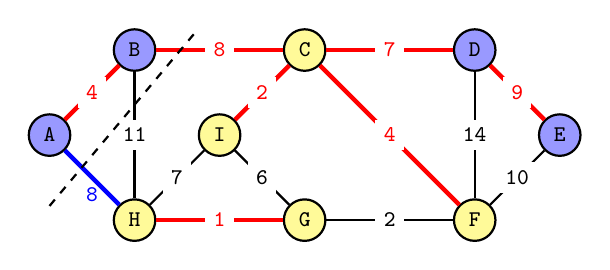
\begin{tikzpicture}[
        scale=0.9,
        transform shape,
        thick,
        font=\ttfamily\bfseries\small
    ]
    \tikzset{
        mynodea/.style = {circle, draw=black, align=center,fill=yellow!40},
        mynodeb/.style = {circle, draw=black, align=center,fill=blue!40},
        myedge/.style = {midway, fill=white},
        edgen/.style = {-},
        edger/.style = {-, ultra thick, red},
        edgeb/.style = {-, ultra thick, blue},
    }
        \node[mynodeb] at (0.0,1.2) (a) {A};
        \node[mynodeb] at (1.2,2.4) (b) {B};
        \node[mynodeb] at (6.0,2.4) (d) {D};
        \node[mynodea] at (3.6,2.4) (c) {C};
        \node[mynodea] at (1.2,0.0) (h) {H};
        \node[mynodea] at (3.6,0.0) (g) {G};
        \node[mynodea] at (6.0,0.0) (f) {F};
        \node[mynodea] at (2.4,1.2) (i) {I};
        \node[mynodeb] at (7.2,1.2) (e) {E};
        %
        \draw[edger] (a) edge node[myedge] {4} (b);
        \draw[edger] (b) edge node[myedge] {8} (c);
        \draw[edger] (c) edge node[myedge] {7} (d);
        \draw[edger] (d) edge node[myedge] {9} (e);
        %
        \draw[edgeb] (a) edge node[below] {8} (h);
        \draw[edger] (h) edge node[myedge] {1} (g);
        \draw[edgen] (g) edge node[myedge] {2} (f);
        \draw[edgen] (f) edge node[myedge] {10} (e);
        %
        \draw[edgen] (h) edge node[myedge] {7} (i);
        \draw[edgen] (i) edge node[myedge] {6} (g);
        \draw[edger] (i) edge node[myedge] {2} (c);
        %
        \draw[edgen] (b) edge node[myedge] {11} (h);
        \draw[edgen] (d) edge node[myedge] {14} (f);
        \draw[edger] (c) edge node[myedge] {4} (f);

        \path[draw,dashed] (0.0,0.2) -- (2.1,2.7);
    \end{tikzpicture}
\end{page}

\begin{page}
    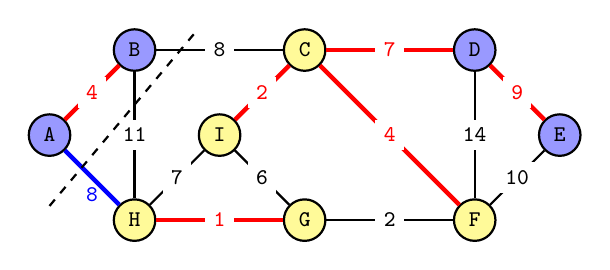
\begin{tikzpicture}[
        scale=0.9,
        transform shape,
        thick,
        font=\ttfamily\bfseries\small
    ]
    \tikzset{
        mynodea/.style = {circle, draw=black, align=center,fill=yellow!40},
        mynodeb/.style = {circle, draw=black, align=center,fill=blue!40},
        myedge/.style = {midway, fill=white},
        edgen/.style = {-},
        edger/.style = {-, ultra thick, red},
        edgeb/.style = {-, ultra thick, blue},
    }
        \node[mynodeb] at (0.0,1.2) (a) {A};
        \node[mynodeb] at (1.2,2.4) (b) {B};
        \node[mynodeb] at (6.0,2.4) (d) {D};
        \node[mynodea] at (3.6,2.4) (c) {C};
        \node[mynodea] at (1.2,0.0) (h) {H};
        \node[mynodea] at (3.6,0.0) (g) {G};
        \node[mynodea] at (6.0,0.0) (f) {F};
        \node[mynodea] at (2.4,1.2) (i) {I};
        \node[mynodeb] at (7.2,1.2) (e) {E};
        %
        \draw[edger] (a) edge node[myedge] {4} (b);
        \draw[edgen] (b) edge node[myedge] {8} (c);
        \draw[edger] (c) edge node[myedge] {7} (d);
        \draw[edger] (d) edge node[myedge] {9} (e);
        %
        \draw[edgeb] (a) edge node[below] {8} (h);
        \draw[edger] (h) edge node[myedge] {1} (g);
        \draw[edgen] (g) edge node[myedge] {2} (f);
        \draw[edgen] (f) edge node[myedge] {10} (e);
        %
        \draw[edgen] (h) edge node[myedge] {7} (i);
        \draw[edgen] (i) edge node[myedge] {6} (g);
        \draw[edger] (i) edge node[myedge] {2} (c);
        %
        \draw[edgen] (b) edge node[myedge] {11} (h);
        \draw[edgen] (d) edge node[myedge] {14} (f);
        \draw[edger] (c) edge node[myedge] {4} (f);

        \path[draw,dashed] (0.0,0.2) -- (2.1,2.7);
    \end{tikzpicture}
\end{page}

\begin{page}
    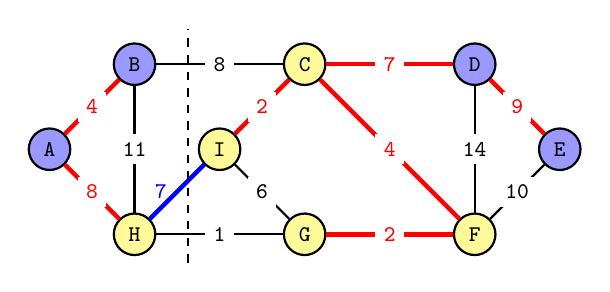
\begin{tikzpicture}[
        scale=0.9,
        transform shape,
        thick,
        font=\ttfamily\bfseries\small
    ]
    \tikzset{
        mynodea/.style = {circle, draw=black, align=center,fill=yellow!40},
        mynodeb/.style = {circle, draw=black, align=center,fill=blue!40},
        myedge/.style = {midway, fill=white},
        edgen/.style = {-},
        edger/.style = {-, ultra thick, red},
        edgeb/.style = {-, ultra thick, blue},
    }
        \node[mynodeb] at (0.0,1.2) (a) {A};
        \node[mynodeb] at (1.2,2.4) (b) {B};
        \node[mynodeb] at (6.0,2.4) (d) {D};
        \node[mynodea] at (3.6,2.4) (c) {C};
        \node[mynodea] at (1.2,0.0) (h) {H};
        \node[mynodea] at (3.6,0.0) (g) {G};
        \node[mynodea] at (6.0,0.0) (f) {F};
        \node[mynodea] at (2.4,1.2) (i) {I};
        \node[mynodeb] at (7.2,1.2) (e) {E};
        %
        \draw[edger] (a) edge node[myedge] {4} (b);
        \draw[edgen] (b) edge node[myedge] {8} (c);
        \draw[edger] (c) edge node[myedge] {7} (d);
        \draw[edger] (d) edge node[myedge] {9} (e);
        %
        \draw[edger] (a) edge node[myedge] {8} (h);
        \draw[edgen] (h) edge node[myedge] {1} (g);
        \draw[edger] (g) edge node[myedge] {2} (f);
        \draw[edgen] (f) edge node[myedge] {10} (e);
        %
        \draw[edgeb] (h) edge node[left] {7} (i);
        \draw[edgen] (i) edge node[myedge] {6} (g);
        \draw[edger] (i) edge node[myedge] {2} (c);
        %
        \draw[edgen] (b) edge node[myedge] {11} (h);
        \draw[edgen] (d) edge node[myedge] {14} (f);
        \draw[edger] (c) edge node[myedge] {4} (f);

        \path[draw,dashed] (1.95,-0.4) -- (1.95, 2.9);
    \end{tikzpicture}
\end{page}

\end{document}
\end{figure}

% \phantom{\lipsum}

\begin{algorithm}[H]
	\caption{Cammini Minimi}
	\documentclass[varwidth=6in]{standalone}
\usepackage{../_preamble}

% arara: pdflatex: { synctex: no }
% arara: latexmk: { clean: partial }
\begin{document}
\ifstandalone
\NoCaptionOfAlgo
\begin{algorithm}[H]
\caption[Algoritmo di Kruskal]{}
\fi

\prototype{\Set \kruskal{\Edge{} \(A\), \Int \(n\), \Int \(m\)}}{
\tcp{\Edge{}: vettore di archi}

	\BlankLine
	\lnl{kruskal:init}%
	\Set \(T\) \Assign \setConstructor \Comment*[h]{insieme (inizialmente vuoto) che conterrà gli archi dell'albero minimo}\;
	\mfSet \(M\) \Assign \mfConstructor{n} \Comment*[h]{insieme disgiunto grande }\;

	\BlankLine
	\tcp{ordino per peso crescente}
	\lnl{kruskal:order}%
	\{ ordina \ArrayCall{A}{1}{m} in modo che \(\ArrayCall{A}{1}.\peso \leqslant \cdots \leqslant \ArrayCall{A}{m}.\peso\) \}\;
%
	\BlankLine
	\Int \(c \Assign 0\) \Comment*[h]{quanti archi ho aggiunto}\;
	\Int \(i \Assign 1\) \Comment*[h]{quale arco sto guardando}\;
	\lnl{kruskal:op}%
	\While(\Comment*[h]{Termina quando l'albero è costruito}){\(c < n-1\) \And \(i \leqslant m\)}{
%
		\BlankLine
		\tcp{\(c < n-1\): ho raggiunto tutti gli archi necessari per fare un albero}
		\tcp{\(i \leqslant m\): ho esaurito tutti gli archi da guardare (per controllo)}
		\If(\Comment*[h]{non fanno parte dello stesso albero}){\(M.\mfFind{\(A[i].u\)} \Neq M.\mfFind{\(A[i].v\)}\)}{

			\BlankLine
			\(M.\mfMerge{\(A[i].u\), \(A[i].v\)}\) \Comment*[l]{unisco gli insiemi disgiunti}
			\(T.\setInsert{\(A[i]\)}\) \Comment*[l]{inserisco l'arco all'albero}
			\(c \Assign c + 1\) \Comment*[l]{ho aggiunto un altro arco}
		}

		\BlankLine
		\(i \Assign i + 1\) \Comment*[l]{guardo il prossimo arco}
	}

	\Return \(T\) \Comment*[l]{Ritorna l'albero di copertura minimo}
}

\ifstandalone
\end{algorithm}
\RestoreCaptionOfAlgo
\fi
\end{document}

	%&../preamble

% arara: pdflatex: { synctex: no }
% arara: latexmk: { clean: partial }
\ifstandalone
\begin{document}
\begin{algorithm}[H]
\fi

\prototype{\prim{\Graph \(G\), \Node \(r\), \Array{\Int} \(p\)}}{
	\tcp{\(r\): nodo dalla quale parto}
	\tcp{\(p\): vettore dei padri}

	\BlankLine
	\Heap \(Q\) \Assign \minHeapConstructor\;
	\PriorityItem{} \Pos \Assign \new \PriorityItem{1\dots G.n}\;

	\BlankLine
	% \tcp{Per ciascun nodo appartenente al grafo, esclusa la radice che ne fa già parte}
	\tcp{inserisco i nodi nella coda, memorizzando la loro posizione}
	\lnlset{prim:init}{1}%
	\ForEach{\(u \in G.\VV() - \{ r \}\)}{
		% \tcp{li inserisco, memorizzando la loro posizione, nella coda indicando che devono ancora essere raggiunti (\(+\infty\))}
		\(\Pos[u] \Assign Q.\heapInsert(u, +\infty)\)\;
	}

	\BlankLine
	\tcp{Inserisco il "nodo di partenza"}
	\(\Pos[r] \Assign Q.\heapInsert{r, 0}\)\;
	\(p[r] \Assign 0\) \Comment*[l]{convenzione per indicare che non ha padre}

	\BlankLine
	\lnlset{prim:ciclo-esterno}{2}%
	\While(\Comment*[h]{non ci sono più nodi}){\Not \(Q\).\setEmpty}{

	\BlankLine
		\Node \(u\) \Assign \(Q\).\heapDeleteMin \Comment*[l]{cancello e restituisco il nodo}
		\(\Pos[u] \Assign \Nil\) \Comment*[h]{non considero più quel nodo}\;

		\BlankLine
		\tcp{per ciascun nodo adiacente a quello considerato}
		\lnlset{prim:ciclo-interno}{3}%
		\ForEach{\(v \in G.\adj(u)\)}{

			\BlankLine
			\If{\(\Pos[v] \Neq \Nil\) \And \(\weight{u,v} < \Pos[v].\priority\)}{
				\tcp{\(\Pos[v] \Neq \Nil\): è già stato visitato}
				\tcp{\(\weight{u,v} < \Pos[v].\priority\): }

				\BlankLine
				\(Q.\heapDecrease{\Pos[v], \weight{u,v}}\) \Comment*[l]{commento}
				\(p[v] \Assign u\) \Comment*[l]{commento}
			}
		}
	}
}

\ifstandalone
\end{algorithm}
\end{document}
\fi

	\documentclass[varwidth=6in]{standalone}
\usepackage{../_preamble}

% arara: pdflatex: { synctex: no }
% arara: latexmk: { clean: partial }
\begin{document}
\ifstandalone
\NoCaptionOfAlgo
\begin{algorithm}[H]
\caption[Algoritmo di Dijkstra]{}
\fi

\prototype{\Array{\Int}, \Array{\Int} \CamminiMinimi{\Graph \(G\), \Node \(s\)}}{

	\BlankLine
	\lnl{dijkstra:init}%
	\alert{ \Heap \(S\) \Assign \heapConstructor } \Comment*[l]{\(\Omicron(n) \cdot 1\)}
	\alert{ \(S\).\heapInsert{\(s\), \(0\)} }\;

	\BlankLine
	\While(\Comment*[h]{\(\Omicron(n)\)}){\Not \(S.\setEmpty{}\)}{

		\lnl{dijkstra:remove}%
		\tcp{\(\Omicron(n)\) vettore ordinato / \(\Omicron(\log n)\) heap binario}
		\alert{\Int \(u\) \Assign \(S\).\heapDeleteMin }\;
		\ArrayCall{b}{u} \Assign \False\;
	%
		\BlankLine
		\ForEach{\( v \in G.\adj{u} \)}{
			\If{\( \ArrayCall{d}{u} + G.\weight{u,v} < \ArrayCall{d}{v} \)}{

				\BlankLine
				\eSea{\(\Not \ArrayCall{b}{v}\)}{
					\lnl{dijkstra:add}%
					\tcp{\(\Omicron(1) \cdot n\) vettore ordinato / \(\Omicron(\log n) \cdot n\) heap binario}
					% \alert{ \(S.\heapInsert{\(v\), \(\ArrayCall{d}{u} + G.\weight{u,v}\)}\)} \;
					\ArrayCall{b}{v} \Assign \True\;
				}{
					\lnl{dijkstra:update}%
					\tcp{\(\Omicron(1) \cdot m\) vettore ordinato / \(\Omicron(\log n) \cdot m\) heap binario}
					% \alert{ \(S\).\heapDecrease{\(v\), \(\ArrayCall{d}{u} + G.\weight{u,v}\)} }\;
				}
				\ArrayCall{T}{v} \Assign \(u\)\;
				\ArrayCall{d}{v} \Assign \(\ArrayCall{d}{u} + G.\weight{u,v}\)\;
			}
		}
	}
	\Return \((T, d)\)\;
}

\ifstandalone
\end{algorithm}
\RestoreCaptionOfAlgo
\fi
\end{document}

\end{algorithm}

\end{multicols}

\end{document}
